\part{数据库篇}
\chapter{MySQL数据库基本知识}

MySQL\index{MySQL}是一个关系型数据库管理系统,由瑞典MySQL AB公司开发,
目前属于Oracle公司。MySQL是一个命途多舛的产品,2008年2月26日被Sun完全收
购,2009年4月20日Oracle并购了Sun公司。业界一片哗然,一时众说纷纭,褒贬
不一。在此过程中衍生出了两个版本的数据库,一个是Percona
Server及MariaDB,这些版本的衍生,是考虑到Oracle将其闭源的潜在可能。

关系型数据库将数据保存在不同的表中,而不是将所有数据放在一个大仓库内,
这样就增加了速度并提高了灵活性。MySQL所使用的SQL语言是用于访问数据库的
最常用标准化语言。MySQL软件采用了双授权策略,它分为
社区版和商业版,由于其体积小、速度快、总体拥有成本低,尤其是开放源码这
一特点,一般中小型网站的开发都选择MySQL作为其网站的数据库。由于其社区版的性
能卓越,搭配PHP和Apache可组成良好的开发环境。

\section{存储设备配置}

\subsection{构建文件系统}

使用xfs文件系统来提供MySQL数据的存储。使用xfs的话,需要添加管理配置工具
包,如下:

\begin{verbatim}
A0305010:~ # zypper -y install xfsdump xfsprogs   
A0305010:~ # modprobe -v xfs 
insmod /lib/modules/3.0.13-0.27-default/kernel/fs/xfs/xfs.ko
\end{verbatim}

使用mkfs.xfs创建文件系统如下:

\begin{verbatim}
A0305010:~ # fdisk /dev/sdb
Command (m for help): n
Command action
   e   extended
   p   primary partition (1-4)
p
Partition number (1-4, default 1): 
Using default value 1
First sector (2048-121634815, default 2048): 
Using default value 2048
Last sector, +sectors or +size{K,M,G} (2048-121634815, default 121634815): 
Using default value 121634815

Command (m for help): w
The partition table has been altered!

Calling ioctl() to re-read partition table.
Syncing disks.
A0305010:~ # partprobe /dev/sdb
A0305010:~ # mkfs.xfs -f -i size=512,attr=2 -l lazy-count=1 \
> -d su=64k,sw=10 -L /data1 /dev/sdb1
\end{verbatim}

注:这里的sdb是我们使用的一个样例。不同SSD厂商的设备在系统里被识别的标
识不一定是/dev/sdb,根据实际情况选择合适的标示符(如,Fusion-io的设备在
本次测试中被识别为/dev/fioa;LSI的设备在本次测试中被识别
为/dev/sdb;Intel的设备在本次测试中被识别为/dev/nvme0n1;宝存的设备在本
次测试中被识别为/def/dfa)。

\subsection{挂载文件系统}

\begin{verbatim}
A0305010:~ # mkdir /data1
A0305010:~ # cd /data1
A0305010:~ # mkdir mysqldata1 mysqldata2 mysqldata3 mysqldata4
A0305010:~ # mount -t xfs -o defaults,rw,noatime,nodiratime,\
> noikeep,nobarrier,allocsize=8M,attr2,largeio,\
> inode64,swalloc /dev/sdb1  /data1
\end{verbatim}

在/etc/fstab中添加自动挂载参数如下:
\begin{verbatim}
/dev/sdb1  /data1 xfs defaults,rw,noatime,nodiratime,noikeep,nobarrier,allocsize=8M,attr2,largeio,inode64,swalloc  0  0
A0305010:~ # mount -a
\end{verbatim}

\section{安装MySQL}
\subsection{创建MySQL用户}

我们需要添加专门的MySQL用户,并设置它的uid及gid为601。

\small{
\begin{verbatim}
[root@iLiuc ~]# groupadd -g 601 mysql
[root@iLiuc ~]# useradd -c "mysql software owner" -g mysql \
> -u 601 -m -d /home/mysql mysql
\end{verbatim}
}
\normalsize

\subsection{安装MySQL}

采用二进制方案安装,步骤如下:
\begin{enumerate}[itemsep=0pt,parsep=0pt]
\item 首先获取与生产环境数据库相同的二进制安装文件
\begin{verbatim}
A0305010:~ # mkdir /home/mysql/program
A0305010:~ # cd /home/mysql/program
A0305010:~ # ls
p16901968_55_Linux-x86-64.zip
\end{verbatim}
\item 解压
\begin{verbatim}
A0305010:~ # unzip p16901968_55_Linux-x86-64.zip
A0305010:~ # ls
README.txt
keepalived-1.2.7-8.1.x86_64.rpm
mysql-advanced-5.5.32-linux2.6-x86_64.tar.gz
mysql-advanced-5.5.32-linux2.6-x86_64.tar.gz.asc
mysql-advanced-5.5.32-linux2.6-x86_64.tar.gz.md5
p16901968_55_Linux-x86-64.zip
A0305010:~ # tar -xf mysql-advanced-5.5.32-linux2.6-x86_64.tar.gz
\end{verbatim}
\item 创建数据目录
\begin{verbatim}
A0305010:~ # mkdir /home/mysql/data
A0305010:~ # cd /home/mysql/data
A0305010:~ # mkdir conf innodb_log innodb_ts log mydata \
> relaylog slowlog sock tmpdir undo binlog
\end{verbatim}
\item 初始化MySQL元数据
\begin{verbatim}
A0305010:~ # cd /home/mysql/program/mysql-advanced-5.5.32-linux2.6-x86_64
A0305010:~ # ./scripts/mysql_install_db \
> --defaults-file=/home/mysql/conf/my1.cnf \
> --user=mysql \
> --skip-name-resolve
\end{verbatim}
\item 链接到/usr/local/mysql
\begin{verbatim}
A0305010:~ # ln -s /home/mysql/program/mysql-advanced-5.5.32-linux2.6-x86_64 \
> /usr/local/mysql
A0305010:~ # ln -s /data1/mysqldata1 /home/mysql/data/mysqldata1
A0305010:~ # ln -s /data1/mysqldata2 /home/mysql/data/mysqldata2
A0305010:~ # ln -s /data1/mysqldata3 /home/mysql/data/mysqldata3
A0305010:~ # ln -s /data1/mysqldata4 /home/mysql/data/mysqldata4
\end{verbatim}
\end{enumerate}

\small{
\begin{verbatim}
[root@iLiuc ~]# groupadd -g 601 mysql
[root@iLiuc ~]# useradd -c "mysql software owner" -g mysql \
> -u 601 -m -d /home/mysql mysql
\end{verbatim}
}
\normalsize

\section{操作系统配置}
\subsection{进程文件数配置}

由于MySQL采用多线程形式,每个进程打开的文件数要求比较高。所以我们需要增
加ulimit进程文件数的限制。在/etc/rc.local中添加:

\begin{verbatim}
A0305010:~ # /etc/init.d/sshd stop
A0305010:~ # ulimit -HSn 65535
\end{verbatim}

把上述配置写到配置文件/etc/security/limits.conf,找到“\# End of file”,
在其上添加3行

\begin{verbatim}
A0305010:~ # vi /etc/security/limits.conf
* hard memlock unlimited
* soft memlock unlimited
*		-	nofile		65535
A0305010:~ # /etc/init.d/sshd start
\end{verbatim}

\subsection{sysctl配置}

修改sysctl,添加swapness并设置TIME\_WAIT的相关参数。避免内存被交换并且减
少TIME\_WAIT状态时间。

\begin{verbatim}
A0305010:~ # echo "vm.swappiness = 0" >>/etc/sysctl.conf
A0305010:~ # echo "net.ipv4.tcp_tw_reuse=1" >>/etc/sysctl.conf
A0305010:~ # echo "net.ipv4.tcp_tw_recycle=1" >>/etc/sysctl.conf
A0305010:~ # echo "net.ipv4.tcp_fin_timeout = 30" >>/etc/sysctl.conf
A0305010:~ # sysctl -p
\end{verbatim}

\subsection{cgroup配置}

我们只对cpu和内存做限制,所以只需要挂载两个子系统。另外,我们在本服务器
上计划启动4个实例,这四个实例分别属于四个组,mysql\_g1, mysql\_g2,
mysql\_g3, mysql\_g4。目前我们限制它们都在4个超线程并且每个实例的内存不
超过24G。如下:

\begin{verbatim}
A0305010:~ # zypper install -y libcgroup1
A0305010:~ # cat /etc/cgconfig.conf
mount {
    cpuset  = /cgroup/cpuset;
    memory  = /cgroup/memory;
}
group mysql_g1 {
    cpuset {
        cpuset.cpus = 17-20;
        cpuset.mems = 0;
    }
    memory {
        memory.limit_in_bytes=25769803776;
        memory.swappiness=0;
    }
}
group mysql_g2 {
    cpuset {
        cpuset.cpus = 12-16;
        cpuset.mems = 0;
    }
    memory {
        memory.limit_in_bytes=25769803776;
        memory.swappiness=0;
    }
}
group mysql_g3 {
    cpuset {
        cpuset.cpus = 5-8;
        cpuset.mems = 0;
    }
    memory {
        memory.limit_in_bytes=25769803776;
        memory.swappiness=0;
        }
}
group mysql_g4 {
    cpuset {
        cpuset.cpus = 1-4;
        cpuset.mems = 0;
    }
    memory {
        memory.limit_in_bytes=25769803776;
        memory.swappiness=0;
    }
}

A0305010:~ # /etc/init.d/cgconfig start
\end{verbatim}

\subsection{cgrule配置}

我们设置使用mysqld\_safe1启动的命令为mysql\_g1组,这样就可以限制它的CPU和
内存使用。其他的四个实例同样进行设置如下:

\begin{verbatim}
A0305010:~ # cat /etc/cgrules.conf
*:/usr/local/mysql/bin/mysqld_safe1    *    mysql_g1
*:/usr/local/mysql/bin/mysqld_safe2    *    mysql_g2
*:/usr/local/mysql/bin/mysqld_safe3    *    mysql_g3
*:/usr/local/mysql/bin/mysqld_safe4    *    mysql_g4

A0305010:~ # /etc/init.d/cgred start
\end{verbatim}

\section{MySQL配置}
\subsection{程序文件和目录配置}
\subsection{多实例配置}

\begin{enumerate}[itemsep=0pt,parsep=0pt]
\item my.cnf文件配置

  我们在/home/mysql/conf下保存着my1.cnf,my2.cnf,my3.cnf,my4.cnf。针对
  每一个数据库实例都有一个对应的配置文件。各个配置文件中都保存的是每个实
  例独立的配置。通过“实例切换配置”来切换到各个不同的实例。

\item 实例切换配置

  我们在/home/mysql/bin下存放有四个文件my1,my2,my3,my4。用于切换到各
  个实例的配置环境中。并且我们在profile中添加了对应的别名:

\begin{verbatim}
alias my1=". /home/mysql/bin/my1"
alias my2=". /home/mysql/bin/my2"
alias my3=". /home/mysql/bin/my3"
alias my4=". /home/mysql/bin/my4"
\end{verbatim}

  如,my1文件内容如下:

\begin{verbatim}
#!/bin/sh
#****************************************************************#
# ScriptName: my1
#             switch to mysql instance 1 environment
# Author:
# Create Date: 2013-03-27
# Modify Author:
# Modify Date: 2013-03-27
# Function:
#***************************************************************#
#set -x

#### variable should change every instance
export INSTANCE_NO=1

#### variable should change every instance
export MYSQL_PORT=$(expr 3305 + $INSTANCE_NO)
export MYSQL_PROGRAM=/usr/local/mysql
export DATA_DIR=/home/mysql/data/mysqldata$INSTANCE_NO/
export MYSQL_CONF=/home/mysql/conf/my$INSTANCE_NO.cnf
export PS1="\n\e[1;37m[\e[m\e[1;36mMySQL$INSTANCE_NO\e[m \$(date \"+%Y-%m-%d %H:%M:%S\") \e[1;31m\u@\e[m\e[1;31m\h\e[m \e[4m\$(pwd)\e[m\e[1;37m]\e[m\e[1;36m\e[m\n\$"
alias stopmysql="$MYSQL_PROGRAM/bin/mysqladmin --defaults-file=$MYSQL_CONF -uroot -p111111 -hlocalhost -P$MYSQL_PORT shutdown"
alias my="$MYSQL_PROGRAM/bin/mysql --defaults-file=$MYSQL_CONF -uroot -p111111 -hlocalhost -P$MYSQL_PORT test --prompt='[$(whoami)@$(hostname):$(pwd) \\v_Instance$INSTANCE_NO \\u@\\h:\\d \\R:\\m:\\s] >'"

#### variable should not change every version
export PATH=$MYSQL_PROGRAM/bin/:$PATH
export LD_LIBRARY_PATH=$MYSQL_PROGRAM/lib/
export PROMPT_COMMAND='echo -ne "\033]0;${USER}@${HOSTNAME%%.*}"; echo -ne "\007"'

startmysql()
{
	cd $MYSQL_PROGRAM/
	$MYSQL_PROGRAM/bin/mysqld_safe$INSTANCE_NO --defaults-file=${MYSQL_CONF} & cd -
}

alias cdd="cd $DATA_DIR"
alias cdb="cd $MYSQL_PROGRAM"
alias cdm="cd /home/mysql/"
alias cdqm="cd $QGUARD_BASEDIR"
alias vi="vim"
alias vie="vim $DATA_DIR/log/error.log"
alias cate="cat $DATA_DIR/log/error.log"
alias psm="ps -ef|grep $MYSQL_PROGRAM/bin/mysqld |grep -v grep"
alias ll='ls -l -G'
alias rm='rm -i'
alias cp='cp -i'
alias mv='mv -i'
\end{verbatim}

\end{enumerate}

直接输入命令my1就可以切换到mysql实例1的环境下。此时可以直接输入my1命令
登录第一个实例的mysql环境,输入stopmysql就可以停掉MySQL数据库,输
入startmysql就可以启动MySQL数据库。

另外,还做了一些简单方便的命令,以便管理:

\begin{quote}
  cdd用于切换到实例的数据目录
  cdm用于切换到MySQL根目录
  cdb用于切换到MySQL的程序文件目录
  psm用于输出MySQL数据库的进程和cgroup信息等
\end{quote}

\section{数据库日常管理}
\subsection{实例切换}
\subsection{MySQL启动}
\subsection{MySQL关闭}

\section{如何进入MySQL数据库}

进入MySQL数据库很简单,首先确保mysqld进程已经启动。如果没有启动,请参照
前面的命令启动之。只需要在命令行输入命令mysql回车即可,因为我们的IPTV系
统里的mysql的root账户是没有密码的。

\small{
\begin{verbatim}
[root@iLiuc ~]# mysql
mysql> show databases;      <- 查看我们有哪些库
+-------------------------+
| Database                |
+-------------------------+
| information_schema      | 
| clear_360fy             | <- 稍后我们将导出这个库 
| clear_iptv2x            | 
| clear_iptv_Skyworth     | 
| clear_qingpu_school     | 
| clear_vod_mingzhu       | 
| clear_vod_new           | 
| clear_vod_yiyuan        | 
| clear_xianhuashan       | 
| cleardb_str             | 
| happyview               | 
+-------------------------+

mysql> use clear_360fy;     <- 选择要使用的库
Database changed            <- 提示数据库已改变

mysql> show tables;         <- 查看clear_360fy库中有哪些表
+--------------------------+
| Tables_in_clear_360fy    |
+--------------------------+
| config                   | 
| directory                | 
| drinks_info_t            | 
| favorites                | 
| hotel_category           | 
| hotel_info               | 
| language                 | 
| livechannel              | 
| log                      | 
  ...         
| massage                  | 
| program                  | 
| user_group_matrix        | 
| users                    | 
| weather                  | 
| wel_message              | 
+--------------------------+
mysql> exit                 <- 退出数据库
[root@iLiuc ~]# 
\end{verbatim}
}
\normalsize

\section{如何建库建表}

当我们的数据很少时,把这些信息可以手工的记录在纸片上或其他介质上,管理
起来也是很方便的。现如今是信息的时代,我们总不能把数据还是记录在纸上或
龟壳上吧,管理起来非把人给累死。把数据存在易于管理的数据库系统中是明智
之举。

\section{简单sql语句的使用}

有了上面的介绍是不是想动手操练一番。首先确保你的系统中应该安装有mysql数
据软件;其次,要确保mysqld服务已经在运行;最后,要有数据库的用户名及密
码。这里我们使用Clear的用户名及密码为123456为演示环境。

\subsection{create语句的使用}

create可以创建库和表,首先我们以一个具体的例子来演示该命令如何使用。接
下来我们要创建这样一个库,库名为cc(clear company),表的名字为hr(human
resource)

\begin{table}[h]
  \centering
  \begin{tabular}{lrlr}
    \toprule
    id   & name    & deptname       & salary \\
    \midrule
    1    & james   & development    & 1000 \\
    2    & wade    & engineer       & 800 \\
    3    & bosh    & finance        & 600 \\
    4    & richard & sale           & 600 \\
    5    & laven   & it             & 1010 \\
    \bottomrule
  \end{tabular}
\end{table}

\small{
\begin{verbatim}
[root@iLiuc ~]# mysql
mysql> create database if not exists cc;

mysql> use cc;
mysql> create table hr (
       id int not null primary key,
       name char(10) not null,
       deptname char(15) not null,
       salary float(5,2) not null);

mysql> desc hr;
+----------+------------+------+-----+---------+-------+
| Field    | Type       | Null | Key | Default | Extra |
+----------+------------+------+-----+---------+-------+
| id       | int(11)    | NO   | PRI | NULL    |       | 
| name     | char(10)   | NO   |     | NULL    |       | 
| deptname | char(15)   | NO   |     | NULL    |       | 
| salary   | float(5,2) | NO   |     | NULL    |       | 
+----------+------------+------+-----+---------+-------+
\end{verbatim}
}
\normalsize

上面的具体含义,我就不详细讲解了,自己去Google上Baidu一下吧。上面只是把
一个框架给搭建了起来,里面并没有任何数据,我们可以查看一下:

\begin{verbatim}
mysql> select * from hr;
Empty set (0.02 sec) <- 你将会看到这样的提示
\end{verbatim}

\subsection{insert语句的使用}

insert就是往表里面添加数据的,废话不多说,直接看例子:

\small{
\begin{verbatim}
mysql> insert into hr values
       (1, "james", "development", 1000),
       (2, "wade", "engineer", 800),
       (3, "bosh", "finance", 600),
       (4, "richard", "sale", 600),
       (5, "laven", "it", 1010);

mysql> select * from hr;
+----+---------+-------------+--------+
| id | name    | deptname    | salary |
+----+---------+-------------+--------+
|  1 | james   | development | 999.99 | 
|  2 | wade    | engineer    | 800.00 | 
|  3 | bosh    | finance     | 600.00 | 
|  4 | richard | sale        | 600.00 | 
|  5 | laven   | it          | 999.99 | 
+----+---------+-------------+--------+
\end{verbatim}
}
\normalsize

\subsection{select语句的使用}

select应该是数据库中使用最多的命令了,接下来赶紧介绍如何写select语句。

\small{
\begin{verbatim}
[root@iLiuc ~]# mysql -uroot -p123456
mysql> use clear_360fy;
mysql> select * from maincontrol;
...
\end{verbatim}
}
\normalsize

*是通配符,表示所有。上面的语句意思是查看maincontrol表的所有字段。
如果只查看某个字段或某几个字段,该怎么办呢?各字段之间用逗号分开即
可。每个表有哪些字段呢?使用desc查看即可。下面看演示:

\small{
\begin{verbatim}
mysql> desc maincontrol;

mysql> select * from hr;
+----+---------+-------------+--------+
| id | name    | deptname    | salary |
+----+---------+-------------+--------+
|  1 | james   | development | 999.99 | 
|  2 | wade    | engineer    | 800.00 | 
|  3 | bosh    | finance     | 600.00 | 
|  4 | richard | sale        | 600.00 | 
|  5 | laven   | it          | 999.99 | 
+----+---------+-------------+--------+
\end{verbatim}
}
\normalsize

\subsection{update语句的使用}

当有更新的操作时,update命令就派上用场了。当我们忘记信息发布或IPTV后台
的密码时,也是可用用到update语句的,接下来我们看看如何使用。

\small{
\begin{verbatim}
[root@iLiuc ~]# mysql
mysql> use clear_360fy;
mysql> show tables; <- 找到users
mysql> desc users; <- 查看users有哪些字段
+-------------------+
| Field             | 其他列我省略了
+-------------------+
| ID                |
| NAME              | <- 这是用户名
| PASSWORD          | <- 这是密码
| EMAIL             |
| TYPE              |
| 此处省略若干行...
| IDCARD            |
| ADDRESS           |
| TEL               |
+-------------------+

mysql> select name, password from users;
+-------------+----------------------------------+
| name        | password                         |
+-------------+----------------------------------+
| master      | eb0a191797624dd3a48fa681d3061212 | 
| NULL        | aaabf0d39951f3e6c3e8a7911df524c2 | 
| NULL        | 4124bc0a9335c27f086f24ba207a4912 | 
| newmanager  | 81dc9bdb52d04dc20036dbd8313ed055 | 
| firstmanger | 202cb962ac59075b964b07152d234b70 | 
| 123         | 202cb962ac59075b964b07152d234b70 | 
+-------------+----------------------------------+
\end{verbatim}
}
\normalsize

这时,我们看到了后台用户及其密码。密码是使用md5方式加密的,不安全。我们
可以在数据库里查看某个字符串的md5值,如:

\small{
\begin{verbatim}
mysql> select md5("123456");
+----------------------------------+
| md5("123456")                    |
+----------------------------------+
| e10adc3949ba59abbe56e057f20f883e | 
+----------------------------------+
\end{verbatim}
}
\normalsize

发现没有,123456的md5值跟上面master用户密码的md5值一样,那说明
maser用户的密码为123456。即使我们不知道master用户的密码,我们
照样可以在数据库里更新它的密码。这里我们把它的密码改为“654321”,
看操作:

\small{
\begin{verbatim}
mysql> select md5("654321");
+----------------------------------+
| md5("654321")                    |
+----------------------------------+
| c33367701511b4f6020ec61ded352059 | 
+----------------------------------+
\end{verbatim}
}
\normalsize

用鼠标左键选择“c33367701511b4f6020ec61ded352059”,别把双引号也给选上了。
之后按下鼠标中键即可实现粘贴功能

\small{
\begin{verbatim}
mysql> update users set password="c33367701511b4f6020ec61ded352059" 
     > where name="master";
\end{verbatim}
}
\normalsize

或者一步到位:

\small{
\begin{verbatim}
mysql> update users set password=(select md5("654321")) where name="master";
\end{verbatim}
}
\normalsize

再次查询,验证是不是已经改变,这时可以使用新的密码登陆后台了。

\small{
\begin{verbatim}
mysql> select name, password from users where name="master";
+-------------+----------------------------------+
| name        | password                         |
+-------------+----------------------------------+
| master      | c33367701511b4f6020ec61ded352059 | 
+-------------+----------------------------------+
\end{verbatim}
}
\normalsize

\section{数据库文件的备份}

做完一个项目后的第一件事,就是做好现场的备份,包括前台、后台及数据库。
首先,这是一个很好的习惯。如果不这样,万一出现问题,又要重新部署,岂不
是x都碎了。

\subsection{数据库文件的导出}
\label{sec:exportData}

数据库文件的导出,我们这里使用mysqldump命令。别的不多说,直接介绍该命令
如何使用

\begin{verbatim}
[root@iLiuc ~]# mysqldump -u root -p password db_name > db_name.sql
\end{verbatim}

上面这是标准的数据库备份命令,root为数据的用户名,password为root用户的
密码,需要导出的数据库名字为db\_name,然后把数据保存到当前目录下
的db\_name.sql文件。在我们的IPTV系统里,mysql的root账户是没有密码的,如
果我们要备份clear\_360fy的库文件,则输入一下命令即可:

\small{
\begin{verbatim}
[root@iLiuc ~]# mysqldump clear_360fy > /home/clear_360fy.sql
这条命令意思是把clear_360fy的库dump到/home目录下的clear_360fy.sql文件
\end{verbatim}
}
\normalsize

\subsection{数据库文件的导入}
\label{sec:importData}

数据库文件导入的前提是准备要导入的sql文件,这里我们准备好
clear\_360fy.sql文件,然后创建相应的库,再然后把sql文件导入到刚创建的库
中,这里只介绍一种方法,仅供参考。

\small{
\begin{verbatim}
[root@iLiuc ~]# mysqladmin create clear_360fy 
[root@iLiuc ~]# mysql clear_360fy < /home/clear_360fy.sql
\end{verbatim}
}
\normalsize

这条命令意思是先创建clear\_360fy库,然后把/home目录下的clear\_360fy.sql
文件导入到该库中

\section{常用命令总结}

\begin{enumerate}[itemsep=0pt,parsep=0pt]
\item 刷新
\begin{verbatim}
flush privileges;
\end{verbatim}
\item 显示所有数据库
\begin{verbatim}
show databases;
\end{verbatim}
\item 打开数据库
\begin{verbatim}
use dbname;
\end{verbatim}
\item 显示当前数据中所有的表
\begin{verbatim}
show tables;
\end{verbatim}
\item 查看表结构
\begin{verbatim}
desc tables;
\end{verbatim}
\item 删除数据库
\begin{verbatim}
drop database dbname;
\end{verbatim}
\item 删除表
\begin{verbatim}
drop table tbname;
\end{verbatim}
\item 创建数据库
\begin{verbatim}
create database dbname;
\end{verbatim}
\item 查询
\item 查看用户权限
\end{enumerate}

\small{
\begin{verbatim}
# 查询
select 列名称 from 表名称;    

# 查看用户权限
show grants for repl;         

# 查看mysql进程
show processlist;             

# 查看所有用户
select user();                

# 查看主从状态
show slave status\G;          

# 查看所有参数变量
show variables; 

# 查看表的引擎状态
show table status             

# 表存在就删除
drop table if exists user                       

# 表不存在就创建
create table if not exists user                 

# 查询用户权限 先use mysql
select host, user, password from user;          

# 创建表
create table ka(ka_id varchar(6),qianshu int);  

# 查看系统的字符集和排序方式的设定
show variables like 'character_set_%';          

# 查看超时(wait_timeout)
show variables like '%timeout%';                

# 删除空用户
delete from user where user='';                 

# 删除用户
delete from user where user='sss' and host='localhost' ;    

# 改变现有的表使用的存储引擎
alter table mytable engine = MyISAM ;                       

# 查询表引擎
show table status from  库名  where Name='表名';            

# 创建表指定存储引擎的类型(MyISAM或INNODB)
CREATE TABLE innodb (id int, title char(20)) ENGINE = INNODB                     

# 创建主从复制用户
grant replication slave on *.* to '用户'@'%' identified by '密码';               

# 添加索引
ALTER TABLE player ADD INDEX weekcredit_faction_index (weekcredit, faction);     

# 插入字段
alter table name add column accountid(列名)  int(11) NOT NULL(字段不为空);       

# 更新数据
update host set monitor_state='Y',hostname='username' where ip='192.168.1.1';     

# 清除二进制文件
purge binary logs to 'mysql-bin.000051';
\end{verbatim}
}
\normalsize

\subsection{忘记MySQL密码}
\label{sec:ForgotMysqlPass}

如果MySQL正在运行,首先停掉服务,然后终止进程;在安全模式下进入mysql数
据库去修改密码,最后重启mysqld服务。具体操作为:

\begin{verbatim}
# service mysqld stop
# killall -TERM mysqld
# mysqld_safe --skip-grant-tables &
# mysql
mysql> use mysql;
mysql> update user set password('new_pass') where user="root";
mysql> exit
# service mysqld restart
\end{verbatim}

\chapter{MySQL复制}

主服务器/从服务器设置增加了健壮性。主服务器出现问题时,可以切换到从服务
器。

通过在主服务器和从服务器之间切分处理客户查询的负荷,可以得到更好的客户
响应时间。SELECT查询可以发送到从服务器以降低主服务器的查询处理负荷。但
修改数据的语句仍然应发送到主服务器,以便主服务器和从服务器保持同步。

MySQL提供了数据库的同步功能,这对实现数据库的冗灾、备份、恢复、负载均衡
等都是有极大帮助的。

\section{复制如何工作}

MySQL复制数据,总的来说,有三个步骤:

\begin{enumerate}[itemsep=0pt,parsep=0pt]
\item 在主库上把数据更改记录到二进制日志(Binary Log)中(这些记录被称为
  二进制日志事件)。
\item 备库将主库上的日志复制到自己的中继日志(Relay Log)中。
\item 备库读取中继日志中的事件,将其重放到备库数据之上。
\end{enumerate}

复制如何工作:
\begin{figure}[!h]
\centering
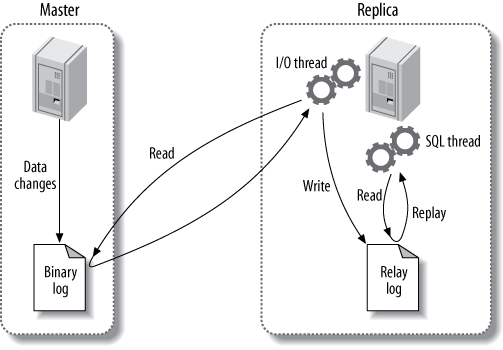
\includegraphics{img/mysql_replication_works}
\caption{MySQL复制的工作原理}
\label{fig:mysqlReplicationWorks}
\end{figure}

第一步是在主库上记录二进制日志。在每次准备提交事务完成数据更新前,主库
将数据更新的事件记录到二进制日志中。MySQL会按事务提交的顺序而非每条语句
的执行顺序来记录二进制日志。在记录二进制日志后,主库会告诉存储引擎可以
提交事务了。

下一步,备库将主库的二进制日志复制到其本地的中继日志中。首先,备库会启
动一个工作线程,称为I/O线程,I/O线程跟主库建立一个普通的客户端连接,然
后在主库上启动一个特殊的二进制转储(binlog dump)线程(该线程没有对应
的SQL命令),这个二进制转储线程会读取主库上二进制日志中的事件。它不会对
事件进行轮询。如果该线程追赶上了主库,它将进入睡眠状态,直到主库发送信
号量通知其有新的事件产生时才会被唤醒,备库I/O线程会将接收到的事件记录到
中继日志中。

备库的SQL线程执行最后一步,该线程从中继日志中读取事件并在备库执行,从而
实现备库数据的更新。当SQL线程追赶上I/O线程时,中继日志通常已经在系统缓
存中了,所以中继日志的开销很低。SQL线程执行的事件也可以通过配置选项来决
定是否写入其自己的二进制日志中。

这种复制架构实现了获取事件的重放事件的解耦,允许这两个过程异步进行。也
就是说I/O线程能够独立于SQL线程之外工作。但这种架构也限制了复制的过程,
其中最重要的一点是在主库上并发运行的查询在备库上只能串化执行,因为只有
一个SQL线程来重放中继日志的事件。

\section{MySQL复制原理}

MySQL支持单向、双向复制、异步复制,复制过程中一个服务器充当主服务器,而
一个或多个其他服务器充当从服务器。主服务器将更新写入一个二进制日志文件
中,并创建一个索引文件以跟踪日志循环。这些日志文件可以将记录发送到从服
务器以让从服务器保持与主服务器的数据一致。当一个从服务器连接主服务器时,
日志文件会通知主服务器,从服务器在上次成功更新的位置处开始进入更新操作。
更新完成后从服务器开始进入等待状态,等待主服务器后续的更新。

\section{MySQL同步细节}

MySQL同步功能由3个线程(Master上1个binlog dump,Slave上2个,分别是SQL进
程和IO进程)来实现。执行“START SLAVE”语句后,Slave就创建

\section{MySQL半同步配置}

\begin{enumerate}[itemsep=0pt,parsep=0pt]
\item 检查是否支持动态加载

登录MySQL并查询have\_dynamic\_loading变量
\begin{verbatim}
mysql_master> show variables like  'have_dynamic_loading';
mysql_slave> show variables like  'have_dynamic_loading';
+----------------------+-------+
| Variable_name        | Value |
+----------------------+-------+
| have_dynamic_loading | YES   |
+----------------------+-------+
1 row in set (0.00 sec)
\end{verbatim}
\item 确认lib/plugin目录下有半同步插件so

  确认主库MySQL程序目录下有lib/plugin/semisync\_master.so文件,确认备
  库MySQL程序目录下有lib/plugin/semisync\_slave.so文件

\begin{verbatim}
ls /usr/local/mysql/lib/plugin
adt_null.so           auth.so               auth_test_plugin.so    
daemon_example.ini    libdaemon_example.so  qa_auth_client.so     
qa_auth_server.so     semisync_slave.so     audit_log.so          
auth_socket.so        authentication_pam.so debug               
mypluglib.so          qa_auth_interface.so  semisync_master.so
thread_pool.so
\end{verbatim}

\item 主库动态加载半同步插件

登录MySQL并加载主库半同步插件,并设置主库半同步有效
\begin{verbatim}
mysql_master> INSTALL PLUGIN rpl_semi_sync_master SONAME 'semisync_master.so';
mysql_master> set global rpl_semi_sync_master_enabled=on
mysql_master> set global rpl_semi_sync_master_timeout=1000
\end{verbatim}
\item 备库动态加载半同步插件
\begin{verbatim}
mysql_slave> INSTALL PLUGIN rpl_semi_sync_slave SONAME 'semisync_slave.so';
mysql_slave> set global rpl_semi_sync_slave_enabled=on; 
\end{verbatim}
\item 主库MySQL配置文件修改

为了保证主库MySQL再次重启服务器后自动打开半同步,需要增加主库MySQL配置如下:
\begin{verbatim}
rpl_semi_sync_master_enabled=1
rpl_semi_sync_master_timeout=1000
\end{verbatim}
\item 备库MySQL配置文件修改

为了保证备库MySQL再次重启服务器后自动打开半同步,需要增加备库MySQL配置如下:
\begin{verbatim}
rpl_semi_sync_slave_enabled=1
\end{verbatim}
\item 备库MySQL重新连接

为了保证主备库是以半同步方式复制的,建议备库上重启复制:
\begin{verbatim}
root@slave >stop slave ; start slave;
\end{verbatim}
\end{enumerate}

\chapter{MySQL+KeepAlived}

\section{KeepAlived介绍}
Keepalived is a routing software written in C. The main goal of this
project is to provide simple and robust facilities for loadbalancing
and high-availability to Linux system and Linux based
infrastructures. Loadbalancing framework relies on well-known and
widely used Linux Virtual Server (IPVS) kernel module providing Layer4
loadbalancing. Keepalived implements a set of checkers to dynamically
and adaptively maintain and manage loadbalanced server pool according
their health. On the other hand high-availability is achieved by VRRP
protocol. VRRP is a fundamental brick for router failover. In
addition, Keepalived implements a set of hooks to the VRRP finite
state machine providing low-level and high-speed protocol
interactions. Keepalived frameworks can be used independently or all
together to provide resilient infrastructures.

使用MySQL双master+keepalived是一种非常好的解决方案,在MySQL-HA环境
中,MySQL互为主从关系,这样就保证了两台MySQL数据的一致性,然后
用KeepAlived实现虚拟IP,通过KeepAlived自带的服务监控功能来实现MySQL故障
时自动切换。

\begin{verbatim}
环境:
mysql_01: 
hostname A0304010 172.16.25.39

mysql_02:
hostname A0305010 172.16.25.40

各个主机授权:
mysql_01> grant replication slave on *.* to 'repl01'@'%' identified by 'replpass';
mysql_01> flush privileges;

mysql_02> grant replication slave on *.* to 'repl02'@'%' identified by 'replpass';
mysql_02> flush privileges;

查看各主机的日志文件及日志位置:
mysql_01> show master status\G
*************************** 1. row ***************************
            File: mysql-bin.000076
        Position: 346
    Binlog_Do_DB: 
Binlog_Ignore_DB: 
1 row in set (0.00 sec)

mysql_02> show master status\G
*************************** 1. row ***************************
            File: mysql-bin.000076
        Position: 346
    Binlog_Do_DB: 
Binlog_Ignore_DB: 
1 row in set (0.00 sec)

各主机change master to:
mysql_01> change master to
    -> master_host='172.16.25.40',
    -> master_user='repl02',
    -> master_password='replpass',
    -> master_port=3313,
    -> master_log_file='mysql-bin.000076',
    -> master_log_pos=346;
Query OK, 0 rows affected (0.35 sec)

mysql_01> start slave;
mysql_01> show slave status\G
*************************** 1. row ***************************
               Slave_IO_State: Waiting for master to send event
                  Master_Host: 172.16.25.40
                  Master_User: repl02
                  Master_Port: 3313
                Connect_Retry: 60
              Master_Log_File: mysql-bin.000076
          Read_Master_Log_Pos: 346
               Relay_Log_File: mysql-relay-bin.000002
                Relay_Log_Pos: 253
        Relay_Master_Log_File: mysql-bin.000076
             Slave_IO_Running: Yes
            Slave_SQL_Running: Yes
              Replicate_Do_DB: 
          Replicate_Ignore_DB: 
           Replicate_Do_Table: 
       Replicate_Ignore_Table: 
      Replicate_Wild_Do_Table: 
  Replicate_Wild_Ignore_Table: 
                   Last_Errno: 0
                   Last_Error: 
                 Skip_Counter: 0
          Exec_Master_Log_Pos: 346
              Relay_Log_Space: 409
              Until_Condition: None
               Until_Log_File: 
                Until_Log_Pos: 0
           Master_SSL_Allowed: No
           Master_SSL_CA_File: 
           Master_SSL_CA_Path: 
              Master_SSL_Cert: 
            Master_SSL_Cipher: 
               Master_SSL_Key: 
        Seconds_Behind_Master: 0
Master_SSL_Verify_Server_Cert: No
                Last_IO_Errno: 0
                Last_IO_Error: 
               Last_SQL_Errno: 0
               Last_SQL_Error: 
  Replicate_Ignore_Server_Ids: 
             Master_Server_Id: 4008
1 row in set (0.00 sec)

mysql_02> change master to 
master_host='172.16.25.39', 
master_useser='repl01', 
master_password='replpass', 
master_port=3313, 
master_log_file='mysql-bin.000076', 
master_log_pos=346;
Query OK, 0 rows affected (0.20 sec)

mysql_02> start slave;
mysql_02> show slave status\G
*************************** 1. row ***************************
               Slave_IO_State: Waiting for master to send event
                  Master_Host: 172.16.25.39
                  Master_User: repl01
                  Master_Port: 3313
                Connect_Retry: 60
              Master_Log_File: mysql-bin.000076
          Read_Master_Log_Pos: 346
               Relay_Log_File: mysql-relay-bin.000002
                Relay_Log_Pos: 253
        Relay_Master_Log_File: mysql-bin.000076
             Slave_IO_Running: Yes
            Slave_SQL_Running: Yes
              Replicate_Do_DB: 
          Replicate_Ignore_DB: 
           Replicate_Do_Table: 
       Replicate_Ignore_Table: 
      Replicate_Wild_Do_Table: 
  Replicate_Wild_Ignore_Table: 
                   Last_Errno: 0
                   Last_Error: 
                 Skip_Counter: 0
          Exec_Master_Log_Pos: 346
              Relay_Log_Space: 409
              Until_Condition: None
               Until_Log_File: 
                Until_Log_Pos: 0
           Master_SSL_Allowed: No
           Master_SSL_CA_File: 
           Master_SSL_CA_Path: 
              Master_SSL_Cert: 
            Master_SSL_Cipher: 
               Master_SSL_Key: 
        Seconds_Behind_Master: 0
Master_SSL_Verify_Server_Cert: No
                Last_IO_Errno: 0
                Last_IO_Error: 
               Last_SQL_Errno: 0
               Last_SQL_Error: 
  Replicate_Ignore_Server_Ids: 
             Master_Server_Id: 3908
1 row in set (0.00 sec)

\end{verbatim}
\section{测试同步}

\begin{verbatim}
mysql_01> show databases;
+--------------------+
| Database           |
+--------------------+
| information_schema |
| mysql              |
| performance_schema |
| sbtest             |
| test               |
+--------------------+
5 rows in set (0.00 sec)

mysql_02> show databases;
+--------------------+
| Database           |
+--------------------+
| information_schema |
| mysql              |
| performance_schema |
| sbtest             |
| test               |
+--------------------+
5 rows in set (0.00 sec)

mysql_01> create database doublec;
mysql_02> show databases;
+--------------------+
| Database           |
+--------------------+
| information_schema |
| liucc              |
| mysql              |
| performance_schema |
| sbtest             |
| test               |
+--------------------+
6 rows in set (0.00 sec)

mysql_02> drop database doublec;
mysql_01> show databases;
+--------------------+
| Database           |
+--------------------+
| information_schema |
| mysql              |
| performance_schema |
| sbtest             |
| test               |
+--------------------+
5 rows in set (0.00 sec)
\end{verbatim}

\section{安装配置KeepAlived}
\begin{verbatim}
安装配置keepalived:
A0304010:
rpm -qa |grep keepalived
keepalived-1.2.7-8.1

cat /etc/keepalived/keepalived.conf
! Configuration File for keepalived

global_defs {
   router_id LVS_DEVEL
}

vrrp_instance MySQL_Loadblancing {
    state BACKUP
    interface vlan0
    virtual_router_id 7
    priority 250
    advert_int 1
    nopreempt
    authentication {
        auth_type PASS
        auth_pass 1111
    }
    virtual_ipaddress {
        172.16.25.7
    }
}

virtual_server 172.16.25.7 3313 {
    delay_loop 6
    lb_algo wrr
    lb_kind DR
    protocol TCP
    persistence_timeout 50

    real_server 172.16.25.39 3313 {
        weight 3
        notify_down /home/mysql/bin/kill_keepalived.sh
        TCP_CHECK {
            connect_timeout 3
            nb_get_retry 3
            delay_before_retry 3
            connect_port 3306
        }
    }
}  

cat /home/mysql/bin/kill_keepalived.sh
#!/bin/bash
pkill keepalived


A0305010:
rpm -qa |grep keepalived
keepalived-1.2.7-8.1

cat /etc/keepalived/keepalived.conf
! Configuration File for keepalived

global_defs {
   router_id LVS_DEVEL
}

vrrp_instance MySQL_Loadblancing {
    state BACKUP
    interface vlan0
    virtual_router_id 7
    priority 200
    advert_int 1
    authentication {
        auth_type PASS
        auth_pass 1111
    }
    virtual_ipaddress {
        172.16.25.7
    }
}

virtual_server 172.16.25.7 3313 {
    delay_loop 6
    lb_algo wrr
    lb_kind DR
    protocol TCP
    persistence_timeout 50

    real_server 172.16.25.40 3313 {
        weight 3
        notify_down /home/mysql/bin/kill_keepalived.sh
        TCP_CHECK {
            connect_timeout 3
            nb_get_retry 3
            delay_before_retry 3
            connect_port 3313
        }
    }
}  

cat /home/mysql/bin/kill_keepalived.sh 
#!/bin/bash
pkill keepalived

\end{verbatim}

\section{启动KeepAlived}

\begin{verbatim}
启动keepalived服务,验证VIP:
A0304010:
/etc/init.d/keepalivd start
ip a
......
8: vlan0@bond0: <BROADCAST,MULTICAST,UP,LOWER_UP> mtu 1500 qdisc noqueue state UP 
    link/ether 6c:92:bf:0a:73:e3 brd ff:ff:ff:ff:ff:ff
    inet 172.16.25.39/24 brd 172.16.25.255 scope global vlan0
    inet 172.16.25.7/32 scope global vlan0
    inet6 fe80::6e92:bfff:fe0a:73e3/64 scope link 
       valid_lft forever preferred_lft forever
......

A0304010:
mysql_01> select host, user from mysql.user;
+-----------+--------+
| host      | user   |
+-----------+--------+
| %         | repl   |
| %         | repl01 |
| %         | sbtest |
| localhost | root   |
+-----------+--------+
4 rows in set (0.00 sec)


A0305010:
/etc/init.d/keepalived start
ip a
......
8: vlan0@bond0: <BROADCAST,MULTICAST,UP,LOWER_UP> mtu 1500 qdisc noqueue state UP 
    link/ether 6c:92:bf:0a:53:07 brd ff:ff:ff:ff:ff:ff
    inet 172.16.25.40/24 brd 172.16.25.255 scope global vlan0
    inet6 fe80::6e92:bfff:fe0a:5307/64 scope link 
       valid_lft forever preferred_lft forever
......

在其他机器上,测试VIP的连通性:
A0304006:
ping 172.16.25.7
PING 172.16.25.7 (172.16.25.7) 56(84) bytes of data.
64 bytes from 172.16.25.7: icmp_seq=1 ttl=64 time=0.174 ms
64 bytes from 172.16.25.7: icmp_seq=2 ttl=64 time=0.143 ms
64 bytes from 172.16.25.7: icmp_seq=3 ttl=64 time=0.151 ms
64 bytes from 172.16.25.7: icmp_seq=4 ttl=64 time=0.168 ms
64 bytes from 172.16.25.7: icmp_seq=5 ttl=64 time=0.174 ms
^C
--- 172.16.25.7 ping statistics ---
5 packets transmitted, 5 received, 0% packet loss, time 3998ms
rtt min/avg/max/mdev = 0.143/0.162/0.174/0.012 ms

在其他机器上登陆VIP,进行验证:
A0304002:~ # mysql -h172.16.25.39 -usbtest -P3313 -p
Enter password: 
Welcome to the MySQL monitor.  Commands end with ; or \g.
Your MySQL connection id is 217
Server version: 5.5.32-enterprise-commercial-advanced-log MySQL Enterprise Server - Advanced Edition (Commercial)

Type 'help;' or '\h' for help. Type '\c' to clear the current input statement.

mysql>mysql> use sbtest;
Database changed
mysql> show tables;
+------------------+
| Tables_in_sbtest |
+------------------+
| sbtest1          | 
| sbtest10         | 
| sbtest11         | 
| sbtest12         | 
| sbtest13         | 
| sbtest14         | 
| sbtest15         | 
| sbtest16         | 
| sbtest17         | 
| sbtest18         | 
| sbtest19         | 
| sbtest2          | 
| sbtest20         | 
| sbtest21         | 
| sbtest22         | 
| sbtest23         | 
| sbtest24         | 
| sbtest3          | 
| sbtest4          | 
| sbtest5          | 
| sbtest6          | 
| sbtest7          | 
| sbtest8          | 
| sbtest9          | 
+------------------+
24 rows in set (0.00 sec)


root@A0304010 /data1]
$netstat -antup |grep 3313
tcp        0      0 0.0.0.0:3313            0.0.0.0:*               LISTEN      10896/mysqld        
tcp        0      0 172.16.25.39:45087      172.16.25.40:3313       ESTABLISHED 10896/mysqld        
tcp        0      0 172.16.25.39:3313       172.16.25.40:42982      ESTABLISHED 10896/mysqld        
tcp        0      0 172.16.25.39:3313       172.16.25.32:32845      ESTABLISHED 10896/mysqld        


MySQL8 2014-12-26 12:20:14 root@A0305010 /data1]
$netstat -antup |grep 3313
tcp        0      0 0.0.0.0:3313            0.0.0.0:*               LISTEN      25423/mysqld        
tcp        0      0 172.16.25.40:3313       172.16.25.39:45087      ESTABLISHED 25423/mysqld        
tcp        0      0 172.16.25.40:42982      172.16.25.39:3313       ESTABLISHED 25423/mysqld   

停掉25.39的MySQL:     
[MySQL8 2014-12-26 12:48:32 root@A0304010 /data1]
$netstat -antup |grep 3313
tcp        0      0 172.16.25.39:45087      172.16.25.40:3313       FIN_WAIT2   -                   
tcp        0      0 172.16.25.39:3313       172.16.25.40:42982      TIME_WAIT   -                   
tcp        0      0 172.16.25.39:3313       172.16.25.32:32845      FIN_WAIT2   -     

              
/etc/init.d/keepalived status
Checking for Keepalived daemon                                   unused


故障切换:
172.16.25.36为客户端,连接VIP来进行查询,
首先,停掉25.39的MySQL服务,验证25.39上的keepalived是不是被停掉了。
ip a
......
8: vlan0@bond0: <BROADCAST,MULTICAST,UP,LOWER_UP> mtu 1500 qdisc noqueue state UP 
    link/ether 6c:92:bf:0a:73:e3 brd ff:ff:ff:ff:ff:ff
    inet 172.16.25.39/24 brd 172.16.25.255 scope global vlan0
    inet 172.16.25.7/32 scope global vlan0
    inet6 fe80::6e92:bfff:fe0a:73e3/64 scope link 
       valid_lft forever preferred_lft forever
......

然后,查看25.36客户端的连接情况。
A0304002:~ # mysql -h172.16.25.7 -usbtest -P3313 -p
Enter password: xxxxxx
Welcome to the MySQL monitor.  Commands end with ; or \g.
Your MySQL connection id is 83
Server version: 5.5.32-enterprise-commercial-advanced-log MySQL Enterprise Server - Advanced Edition (Commercial)

Type 'help;' or '\h' for help. Type '\c' to clear the current input statement.

mysql> show databases;
+--------------------+
| Database           |
+--------------------+
| information_schema | 
| sbtest             | 
| test               | 
+--------------------+
3 rows in set (0.00 sec)

mysql> use sbtest;
mysql> show tables;
+------------------+
| Tables_in_sbtest |
+------------------+
| sbtest1          | 
| sbtest10         | 
| sbtest11         | 
| sbtest12         | 
| sbtest13         | 
| sbtest14         | 
| sbtest15         | 
| sbtest16         | 
| sbtest17         | 
| sbtest18         | 
| sbtest19         | 
| sbtest2          | 
| sbtest20         | 
| sbtest21         | 
| sbtest22         | 
| sbtest23         | 
| sbtest24         | 
| sbtest3          | 
| sbtest4          | 
| sbtest5          | 
| sbtest6          | 
| sbtest7          | 
| sbtest8          | 
| sbtest9          | 
+------------------+
24 rows in set (0.00 sec)

mysql> show tables;
ERROR 1053 (08S01): Server shutdown in progress

mysql> show tables;
No connection. Trying to reconnect...
ERROR 2003 (HY000): Can't connect to MySQL server on '172.16.25.7' (113)
ERROR: 
Can't connect to the server

mysql> show tables;
ERROR 2013 (HY000): Lost connection to MySQL server during query
mysql> show tables;
ERROR 2006 (HY000): MySQL server has gone away
No connection. Trying to reconnect...
Connection id:    22
Current database: sbtest

+------------------+
| Tables_in_sbtest |
+------------------+
| sbtest1          | 
| sbtest10         | 
| sbtest11         | 
| sbtest12         | 
| sbtest13         | 
| sbtest14         | 
| sbtest15         | 
| sbtest16         | 
| sbtest17         | 
| sbtest18         | 
| sbtest19         | 
| sbtest2          | 
| sbtest20         | 
| sbtest21         | 
| sbtest22         | 
| sbtest23         | 
| sbtest24         | 
| sbtest3          | 
| sbtest4          | 
| sbtest5          | 
| sbtest6          | 
| sbtest7          | 
| sbtest8          | 
| sbtest9          | 
+------------------+
24 rows in set (0.02 sec)


最后,查看25.40的keepalived状态及连接情况。
ip a
......
8: vlan0@bond0: <BROADCAST,MULTICAST,UP,LOWER_UP> mtu 1500 qdisc noqueue state UP 
    link/ether 6c:92:bf:0a:53:07 brd ff:ff:ff:ff:ff:ff
    inet 172.16.25.40/24 brd 172.16.25.255 scope global vlan0
    inet 172.16.25.7/32 scope global vlan0
    inet6 fe80::6e92:bfff:fe0a:5307/64 scope link 
......


$netstat -antup |grep 3313
tcp        0      0 0.0.0.0:3313            0.0.0.0:*               LISTEN      28723/mysqld        
tcp        0      0 172.16.25.7:3313        172.16.25.32:43533      ESTABLISHED 28723/mysqld        

A0304010:
A0304010:~ # grep -v "^#" /home/mysql/conf/my8.cnf
[client]
loose_default-character-set = utf8
port=3313
socket=/home/mysql/data/mysqldata8/sock/mysql.sock
user=admin

[mysqld]
large-pages
read_only=off
memlock
default-storage-engine = INNODB
character-set-server=utf8
collation = utf8_bin

user=mysql
port=3313
socket=/home/mysql/data/mysqldata8/sock/mysql.sock
pid-file=/home/mysql/data/mysqldata8/sock/mysql.pid
datadir=/home/mysql/data/mysqldata8/mydata
tmpdir=/home/mysql/data/mysqldata8/tmpdir

skip-name-resolve
skip_external_locking

lower_case_table_names=1
event_scheduler=0
back_log=512
default-time-zone='+8:00'

max_connections = 3000
max_connect_errors=99999
max_allowed_packet = 64M
max_heap_table_size = 8M
max_length_for_sort_data = 16k

wait_timeout=172800
interactive_timeout=172800 

net_buffer_length = 8K
read_buffer_size = 2M
read_rnd_buffer_size = 2M
sort_buffer_size = 2M
join_buffer_size = 4M
binlog_cache_size = 2M
 
table_open_cache = 2048
table_definition_cache = 2048
thread_cache_size = 512
tmp_table_size = 8M

query_cache_size=0
query_cache_type=OFF


log-error=/home/mysql/data/mysqldata8/log/error.log
long_query_time = 1
slow_query_log
slow_query_log_file=/home/mysql/data/mysqldata8/slowlog/slow-query.log
log_warnings
log_slow_slave_statements


server-id=03908
log-bin=/home/mysql/data/mysqldata8/binlog/mysql-bin
binlog-format=ROW
max_binlog_size = 512M
expire_logs_days=15
sync_binlog=1
auto_increment_increment=2
auto_increment_offset=2

relay-log=/home/mysql/data/mysqldata8/relaylog/mysql-relay-bin
slave-skip-errors=1022,1032,1062
report-port=3313
log_bin_trust_function_creators=1
log_slave_updates=1


key_buffer_size = 8M
bulk_insert_buffer_size = 8M
myisam_sort_buffer_size = 64M
myisam_max_sort_file_size = 10G
myisam_repair_threads = 1
myisam_recover

innodb_data_home_dir = /home/mysql/data/mysqldata8/innodb_ts
innodb_data_file_path = ibdata1:2048M:autoextend
innodb_file_per_table
innodb_file_format = barracuda
innodb_file_format_max = barracuda
innodb_file_format_check = ON
innodb_strict_mode = 1
innodb_flush_method = O_DIRECT
innodb_autoinc_lock_mode=2

innodb_additional_mem_pool_size = 8M
innodb_buffer_pool_size = 1G
innodb_max_dirty_pages_pct = 75
innodb_adaptive_flushing = ON
innodb_change_buffering = inserts
innodb_old_blocks_time = 1000

innodb_log_group_home_dir = /home/mysql/data/mysqldata8/innodb_log
innodb_log_buffer_size = 64M
innodb_log_file_size = 2000M
innodb_log_files_in_group = 2
innodb_flush_log_at_trx_commit = 1
innodb_support_xa = ON

innodb_thread_concurrency = 32
innodb_lock_wait_timeout = 120
innodb_rollback_on_timeout = 1
transaction_isolation = READ-COMMITTED

innodb_read_io_threads = 4
innodb_write_io_threads = 12
innodb_io_capacity = 40000
innodb_use_native_aio = 1

innodb_purge_threads = 1

[mysqldump]
quick
max_allowed_packet = 2G
default-character-set = utf8

[mysql]
no-auto-rehash
show-warnings
prompt="5.1 \\u@\\h : \\d \\r:\\m:\\s> "
default-character-set = utf8

[myisamchk]
key_buffer = 512M
sort_buffer_size = 512M
read_buffer = 8M
write_buffer = 8M

[mysqlhotcopy]
interactive-timeout

[mysqld_safe]
user=mysql
open-files-limit = 8192

--------------------------------------------------------

A0305010:
$grep -v "^#" /home/mysql/conf/my8.cnf 
[client]
loose_default-character-set = utf8
port=3313
socket=/home/mysql/data/mysqldata8/sock/mysql.sock
user=admin

[mysqld]
large-pages
read_only=off
memlock
default-storage-engine = INNODB
character-set-server=utf8
collation = utf8_bin

user=mysql
port=3313
socket=/home/mysql/data/mysqldata8/sock/mysql.sock
pid-file=/home/mysql/data/mysqldata8/sock/mysql.pid
datadir=/home/mysql/data/mysqldata8/mydata
tmpdir=/home/mysql/data/mysqldata8/tmpdir

skip-name-resolve
skip_external_locking

lower_case_table_names=1
event_scheduler=0
back_log=512
default-time-zone='+8:00'

max_connections = 3000
max_connect_errors=99999
max_allowed_packet = 64M
max_heap_table_size = 8M
max_length_for_sort_data = 16k

wait_timeout=172800
interactive_timeout=172800 

net_buffer_length = 8K
read_buffer_size = 2M
read_rnd_buffer_size = 2M
sort_buffer_size = 2M
join_buffer_size = 4M
binlog_cache_size = 2M
 
table_open_cache = 2048
table_definition_cache = 2048
thread_cache_size = 512
tmp_table_size = 8M

query_cache_size=0
query_cache_type=OFF

log-error=/home/mysql/data/mysqldata8/log/error.log
long_query_time = 1
slow_query_log
slow_query_log_file=/home/mysql/data/mysqldata8/slowlog/slow-query.log
log_warnings
log_slow_slave_statements

server-id=04008
log-bin=/home/mysql/data/mysqldata8/binlog/mysql-bin
binlog-format=ROW
max_binlog_size = 512M
expire_logs_days=15
sync_binlog=1
auto_increment_increment=2
auto_increment_offset=2

relay-log=/home/mysql/data/mysqldata8/relaylog/mysql-relay-bin
slave-skip-errors=1022,1032,1062
report-port=3313
log_bin_trust_function_creators=1
log_slave_updates=1

key_buffer_size = 8M
bulk_insert_buffer_size = 8M
myisam_sort_buffer_size = 64M
myisam_max_sort_file_size = 10G
myisam_repair_threads = 1
myisam_recover

innodb_data_home_dir = /home/mysql/data/mysqldata8/innodb_ts
innodb_data_file_path = ibdata1:2048M:autoextend
innodb_file_per_table
innodb_file_format = barracuda
innodb_file_format_max = barracuda
innodb_file_format_check = ON
innodb_strict_mode = 1
innodb_flush_method = O_DIRECT
innodb_autoinc_lock_mode=2

innodb_additional_mem_pool_size = 8M
innodb_buffer_pool_size = 8M
innodb_max_dirty_pages_pct = 75
innodb_adaptive_flushing = ON
innodb_change_buffering = inserts
innodb_old_blocks_time = 1000

innodb_log_group_home_dir = /home/mysql/data/mysqldata8/innodb_log
innodb_log_buffer_size = 64M
innodb_log_file_size = 2000M
innodb_log_files_in_group = 2
innodb_flush_log_at_trx_commit = 1
innodb_support_xa = ON

innodb_thread_concurrency = 32
innodb_lock_wait_timeout = 120
innodb_rollback_on_timeout = 1
transaction_isolation = READ-COMMITTED

innodb_read_io_threads = 4
innodb_write_io_threads = 12
innodb_io_capacity = 40000
innodb_use_native_aio = 1

innodb_purge_threads = 1

[mysqldump]
quick
max_allowed_packet = 2G
default-character-set = utf8

[mysql]
no-auto-rehash
show-warnings
prompt="5.5 \\u@\\h : \\d \\r:\\m:\\s> "
default-character-set = utf8

[myisamchk]
key_buffer = 512M
sort_buffer_size = 512M
read_buffer = 8M
write_buffer = 8M

[mysqlhotcopy]
interactive-timeout

[mysqld_safe]
user=mysql
open-files-limit = 8192
\end{verbatim}

\chapter{MySQL+LVS}

\chapter{MHA}
\label{chap:mha}

本文介绍如何一步步搭建MHA高可用环境,

\section{实验环境说明}
\label{sec:MHAEnvSpecific}

使用的MySQL版本为5.5.32企业版,MHA版本为0.56版本,三台服务器。

\subsection{SSH无密码通信设置}
\label{sec:SSHSetup}

在所有机器上执行,设置SSH无密码通信:

\begin{verbatim}
# ssh-keygen -t rsa
# ssh-copy-id -i /root/.ssh/id_rsa.pub root@10.10.7.16
# ssh-copy-id -i /root/.ssh/id_rsa.pub root@10.10.7.17
# ssh-copy-id -i /root/.ssh/id_rsa.pub root@10.10.7.201
\end{verbatim}

\section{安装MySQL}
\label{InstallMySQL}

使用二进制的方式安装MySQL,

\section{安装及配置MHA}
\label{sec:InstallMHANode}

安装方式有两种,可以使用源代码编译安装或者使用RPM包进行安装。使用RPM包
安装简单些,本次安装使用RPM包方式进行安装。安装包可以到这
里https://code.google.com/p/mysql-master-ha/downloads/list下载。

\subsection{安装node节点}
\label{sec:InstallNode}

在所有机器上执行,安装mha的node节点,安装依赖包:

\begin{verbatim}
# yum install -y perl-DBD-MySQL
# rpm -ivh mha4mysql-node-0.56-0.el6.noarch.rpm
\end{verbatim}

\subsection{安装manager节点}
\label{sec:InstallManager}

在Slave机器上执行,安装mha的manager节点,

\begin{verbatim}
# yum install -y perl-Config-Tiny
# yum install -y perl-DBD-MySQL
# yum install -y perl-MIME-Lite
# yum install -y perl-Params-Validate
# yum install -y perl-Time-HiRes
# rpm -ivh perl-Mail-Sender-0.8.16-3.el6.noarch.rpm
# rpm -ivh perl-Mail-Sendmail-0.79-12.el6.noarch.rpm
# rpm -ivh perl-Log-Dispatch-2.27-1.el6.noarch.rpm
# rpm -ivh perl-Parallel-ForkManager-0.7.9-1.el6.noarch.rpm
# rpm -ivh mha4mysql-manager-0.56-0.el6.noarch.rpm
\end{verbatim}



